\documentclass[a4paper,12pt]{report}
\usepackage{titlesec}
\usepackage{amssymb}
\usepackage{amsmath}
\usepackage{graphicx}
\usepackage{geometry}
\geometry{a4paper,left=25mm,right=25mm,top=30mm,bottom=30mm}
\usepackage{cite}
\usepackage{booktabs}
\usepackage{array}
\usepackage{caption}
\usepackage{subcaption}
\usepackage{hyperref}
\usepackage{listings}
\usepackage{xcolor}

\titleformat{\chapter}[display]
  {\normalfont\huge\bfseries\centering}
  {\chaptertitlename\ \thechapter}{20pt}{\Huge}

\begin{document}

% ============================================================
%  TITLE PAGE
% ============================================================
\thispagestyle{empty}
\begin{center}
 \huge{\textsc{RTL Implementation of the KCF/MOSSE Visual Tracking Algorithm on FPGA}}
\end{center}
\vspace{0.25cm}
\begin{center}
 \normalsize{\textit{Project report submitted in partial fulfillment of the requirement for the degree of}}
\end{center}
\begin{center}
\large{Bachelor of Technology\\ in \\Electrical and Computer Engineering}
\end{center}
\vspace{0.5cm}
\begin{center}
 \normalsize{Submitted by}
\end{center}
\vspace{0.5cm}
\begin{center}
 \large{Akhil Sriram (Roll No. [2210110134])}
\end{center}
\vspace{0.25cm}
\begin{center}
 \large{Under Supervision of}
\end{center}
\vspace{0.25cm}
\begin{center}
 \large{Dr. Venkatnarayan Hariharan}\\
 \large{Department of Electrical Engineering}\\
\end{center}
\begin{figure}[htbp]
    \centering
        
\includegraphics[width=4in]{End_Term_Report_Template/logonew.jpg}
\end{figure}
\vspace{0.25cm}
\begin{center}
\large{\textbf{Department of Electrical Engineering}}\\
\large{\textbf{School of Engineering}}\\
\large{\textbf{Shiv Nadar Institution of Eminence}}\\
\vspace{0.25cm}
(April 2026)
\end{center}
\pagebreak

% ============================================================
%  CANDIDATE DECLARATION
% ============================================================
\begin{center}
\huge{\textsc{Candidate Declaration}}
\vspace{1cm}
\end{center}
I hereby declare that the thesis entitled ``KCF/MOSSE Visual Tracking Algorithm on FPGA'' submitted for the B. Tech. degree program. This thesis has been written in my own words. I have adequately cited and referenced the original sources.
\vspace{2cm}\\
\begin{minipage}{7cm}

\includegraphics[width=3cm]{End_Term_Report_Template/Akhil_signature.png}\\
(Signature)\\
Akhil Sriram\\
(2210110134)
\end{minipage}
\pagebreak

% ============================================================
%  CERTIFICATE
% ============================================================
\begin{center}
\huge{\textsc{Certificate}}
\vspace{1cm}
\end{center}
It is certified that the work contained in the project report titled ``RTL Design of a KCF Visual Tracker,'' by \textbf{Akhil Sriram} has been carried out under my supervision and that this work has not been submitted elsewhere for a degree.
\vspace{2cm}\\
\begin{minipage}{7cm}
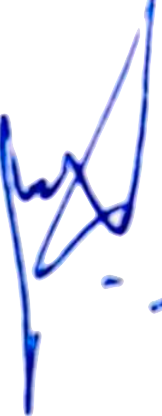
\includegraphics[width=2cm]{End_Term_Report_Template/Venky_signature.png}\\
(Signature)\\
Dr.\ Venkatnarayan Hariharan\\
Dept.\ of Electrical Engineering\\
School of Engineering\\
Shiv Nadar Institution of Eminence\\
Date: \underline{\hspace{3cm}}
\end{minipage}
\pagebreak

% ============================================================
%  ABSTRACT
% ============================================================
\begin{center}
\huge{\textsc{Abstract}}
\end{center}

\vspace{0.5cm}

Visual object tracking is a critical task in computer vision, but traditional software implementations on general-purpose processors often suffer from high latency and power consumption. This project presents a purely hardware-based implementation of the MOSSE (Minimum Output Sum of Squared Error) correlation filter tracking algorithm, designed entirely in Verilog HDL. Unlike software solutions that run sequentially on a CPU, this project leverages the parallel processing capabilities of an FPGA (Field-Programmable Gate Array) to perform high-speed tracking. The design focuses on translating the mathematical operations of the MOSSE algorithm---specifically the Fast Fourier Transforms (FFT) and complex conjugate multiplications---into dedicated digital logic circuits (RTL). The system is designed to operate as a standalone IP core. It accepts image data (such as pixel streams or memory initialization files) as input, processes the frames using a pipeline of custom hardware modules, and outputs the target coordinates. The implementation will be verified through behavioral simulation and synthesized on an FPGA to demonstrate the efficiency and speed advantages of a dedicated hardware solution compared to software-based execution.

\pagebreak
\tableofcontents
\pagebreak
\listoffigures
\pagebreak
\listoftables
\pagebreak

% ============================================================
%  CHAPTER 1: INTRODUCTION
% ============================================================
\chapter{Introduction}

Visual object tracking is the task of continuously estimating the position of a target object across a sequence of video frames, given only its initial location. It is a critical building block for applications including autonomous vehicles, unmanned aerial vehicles (UAVs), surveillance systems, and human-computer interaction. The core challenge lies in handling real-world variations such as illumination changes, partial occlusion, scale variation, and background clutter, while maintaining real-time throughput.

\par General-purpose processors (CPUs) execute tracking algorithms sequentially and are limited by memory bandwidth and clock frequency when processing high-resolution video streams. Field-Programmable Gate Arrays (FPGAs), by contrast, offer massively parallel dataflow architectures, dedicated DSP blocks, and configurable on-chip memory that can be tailored precisely to the arithmetic structure of a given algorithm. This project exploits these properties to implement the KCF tracker as a dedicated hardware IP core.

\section{Background and Motivation}

The demand for real-time tracking in embedded systems has grown significantly. Deployments on edge devices — cameras mounted on drones, robots, or smart infrastructure — impose strict power and latency budgets that general-purpose compute cannot meet. Dedicated FPGA accelerators can achieve an order-of-magnitude improvement in throughput-per-watt compared to equivalent CPU implementations, while remaining reconfigurable unlike ASICs.

\par The Kernelized Correlation Filter \cite{henriques2015} is a particularly strong candidate for hardware acceleration because its dominant operations — the 2D-FFT, element-wise complex multiplication, and 2D-IFFT — map directly to well-understood hardware primitives. All arithmetic is bounded and predictable, making it amenable to fixed-point implementation without requiring floating-point units.

\section{The KCF Approach}

The KCF tracker operates in the frequency domain by treating target patches as cyclic shifts of a base sample. The key insight from Henriques~et~al.\ \cite{henriques2015} is that a matrix of all cyclic shifts of a vector is a \emph{circulant matrix}, and any circulant matrix is diagonalised by the Discrete Fourier Transform (DFT). This means that ridge regression over all cyclic-shift augmented samples reduces to a simple element-wise division in the frequency domain:

\begin{equation}\label{eq:train}
\hat{\alpha} = \frac{\hat{Y}}{|\hat{X}|^2 + \lambda}
\end{equation}

\noindent where $\hat{X} = \mathcal{F}(x)$ is the FFT of the windowed training patch, $\hat{Y} = \mathcal{F}(y)$ is the FFT of the desired Gaussian response label, and $\lambda$ is a regularisation constant. The total computational complexity is $\mathcal{O}(N^2 \log N)$ per frame, compared to $\mathcal{O}(N^6)$ for a naive kernel ridge regression.

\section{Project Scope}

This project implements the KCF tracking pipeline as a synthesisable SystemVerilog IP core with the following parameters and constraints:

\begin{itemize}
    \item Patch size: $N = 32$ pixels (32$\times$32 = 1024 pixels per patch)
    \item Kernel: linear (dot-product kernel; equivalent to standard ridge regression in feature space)
    \item Arithmetic: Q8.8 signed fixed-point (16-bit, 8 fractional bits)
    \item Training: offline — filter coefficients $\hat{\alpha}$ pre-computed in Python and loaded via \texttt{\$readmemh} into on-chip ROM
    \item Detection: online — per-frame pipeline processing live patch data
    \item Interface: AXI4-Stream (pixel ingestion) + AXI4-Lite (control and result registers)
    \item Target hardware: Xilinx Artix-7 XC7A100T (Nexys A7-100T board)
\end{itemize}

% ============================================================
%  CHAPTER 2: LITERATURE SURVEY
% ============================================================
\chapter{Literature Survey}

This chapter surveys the key algorithmic and hardware prior works that directly inform the design decisions made in this project.

\section{MOSSE Filter --- Bolme et al., 2010}

The Minimum Output Sum of Squared Error (MOSSE) filter \cite{bolme2010} was the first correlation-filter-based tracker to demonstrate real-time performance (669~fps). Given a training patch $f$ and desired response $g$, the optimal frequency-domain filter $H^*$ is:

\begin{equation}
H^* = \frac{\sum_i \hat{G}_i \odot \overline{\hat{F}_i}}{\sum_i \overline{\hat{F}_i} \odot \hat{F}_i}
\end{equation}

\noindent where $\hat{G}_i$ and $\hat{F}_i$ are the FFTs of the desired response and training patch respectively, $\overline{(\cdot)}$ denotes complex conjugation, and $\odot$ denotes element-wise multiplication. MOSSE uses a single feature channel (raw grayscale pixels) and a squared loss, which makes it sensitive to illumination changes and appearance variation. The KCF generalises MOSSE by introducing a kernel mapping and multiple feature channels.

\section{KCF Tracker --- Henriques et al., 2015}

The KCF tracker \cite{henriques2015} extends the correlation filter framework to the kernelised (non-linear) setting using the kernel trick. For a Radial Basis Function (RBF) or Gaussian kernel, the dual-space filter coefficients in the frequency domain satisfy:

\begin{equation}
\hat{\alpha} = \frac{\hat{Y}}{\hat{k}^{xx} + \lambda}
\end{equation}

\noindent where $\hat{k}^{xx}$ is the FFT of the kernel correlation between the training patch and itself. For the special case of the linear kernel, $\hat{k}^{xx} = |\hat{X}|^2$ element-wise, which is the formula implemented in this project (see Equation~\ref{eq:train}).

\par A key property exploited by KCF is that the circulant structure of the training data allows the kernel matrix to be diagonalised by the DFT, reducing the $\mathcal{O}(N^4)$ kernel evaluation to $\mathcal{O}(N^2 \log N)$ per frame. This makes real-time operation feasible even on relatively modest hardware.

\section{Normalised Cross-Correlation (NCC) for Target Acquisition}

Normalised Cross-Correlation (NCC) is a classical template-matching technique used in this project for the initial target acquisition step. Given a template $T$ of size $M \times M$ and a search image $I$ of size $P \times P$, the NCC score at position $(r, c)$ is:

\begin{equation}
\text{NCC}(r,c) = \frac{\sum_{i,j} T(i,j) \cdot I(r+i, c+j)}{\sqrt{\sum_{i,j} T(i,j)^2 \cdot \sum_{i,j} I(r+i,c+j)^2}}
\end{equation}

\noindent This can be computed efficiently in $\mathcal{O}(PN \log(PN))$ using the FFT convolution theorem: $\text{corr}(T, I) = \mathcal{F}^{-1}(\overline{\hat{T}} \odot \hat{I})$. In this project, NCC is applied once to locate the target in Frame~2 before handing control to the KCF tracking loop.

\section{Hardware FFT --- Cooley-Tukey Radix-2 DIT}

The Cooley-Tukey algorithm \cite{cooleytukey1965} decomposes an $N$-point DFT into $\log_2 N$ stages of butterfly computations, reducing complexity from $\mathcal{O}(N^2)$ to $\mathcal{O}(N \log_2 N)$. The 2D-FFT is computed by applying the 1D-FFT row-wise and then column-wise (separable row-column decomposition). For $N = 32$, this requires 5 butterfly stages, each accessing precomputed twiddle factor ROMs.

\par Hardware FFT implementations for FPGAs typically use the butterfly unit as the core computation element, with pipelined or iterative architectures depending on the area-throughput tradeoff. This project uses an iterative architecture (\texttt{fft1d\_32.sv}) that computes one butterfly per clock cycle, processing each 32-point FFT in 80 cycles.

\section{Algorithm Comparison}

Table~\ref{tab:algo_compare} summarises the three tracking approaches relevant to this project.

\begin{table}[ht]
\centering
\caption{Comparison of Tracking Algorithms}
\vspace{0.2cm}
\label{tab:algo_compare}
\begin{tabular}{|l|l|l|l|}
\hline
\textbf{Property} & \textbf{NCC} & \textbf{MOSSE} & \textbf{KCF} \\ \hline
Purpose & Acquisition & Tracking & Tracking \\ \hline
Feature Space & Raw pixels & Raw pixels & Linear / RBF kernel \\ \hline
Complexity & $O(MN \log MN)$ & $O(N^2 \log N)$ & $O(N^2 \log N)$ \\ \hline
Robustness & Low & Medium & High \\ \hline
Update Rule & None & Online average & Learning-rate $\eta$ \\ \hline
HW Cost & Medium (1 FFT) & Low (2 FFT) & Medium (6 FFT) \\ \hline
Kernel & None & Linear & Configurable \\ \hline
This Project & Frame 2 only & --- & Frames 3+ \\ \hline
\end{tabular}
\end{table}

% ============================================================
%  CHAPTER 3: WORK DONE
% ============================================================
\chapter{Research and Implementation}

\section{KCF Algorithm Implementation}

\subsection{Training Phase}

Given a $32 \times 32$ training patch $x$ extracted from the first video frame, the offline training procedure computes the KCF filter coefficients $\hat{\alpha}$. The steps are:

\begin{enumerate}
    \item \textbf{Hann Windowing:} Multiply $x$ element-wise by a 2D Hann window to suppress spectral leakage at patch boundaries:
    \begin{equation}
    w[n] = 0.5 - 0.5\cos\!\left(\frac{2\pi n}{N-1}\right), \quad x_w = x \odot (w \otimes w)
    \end{equation}
    \item \textbf{2D-FFT:} Compute $\hat{X} = \mathcal{F}_\text{2D}(x_w)$.
    \item \textbf{Gaussian Label:} Generate a 2D Gaussian response centred at the patch centre:
    \begin{equation}
    y[r,c] = \exp\!\left(-\frac{(r - c_r)^2 + (c - c_c)^2}{2\sigma^2}\right), \quad \hat{Y} = \mathcal{F}_\text{2D}(y)
    \end{equation}
    with $\sigma = 2.0$ pixels and $(c_r, c_c) = (16, 16)$ for a centred $32\times32$ patch.
    \item \textbf{Filter Computation:} Compute the frequency-domain filter coefficients:
    \begin{equation}\label{eq:alpha}
    \hat{\alpha}[k] = \frac{\hat{Y}[k]}{|\hat{X}[k]|^2 + \lambda}, \quad \lambda = 0.01
    \end{equation}
\end{enumerate}

The resulting $\hat{\alpha}$ array (1024 complex Q8.8 values, stored as pairs of 16-bit signed integers) is serialised to \texttt{data/alpha\_hat.mem} using a Python script and loaded into an on-chip ROM at synthesis time via \texttt{\$readmemh}.

\par Figure~\ref{fig:hann} and Figure~\ref{fig:gaussian} show the Hann window applied to a training patch and the corresponding Gaussian label used as the desired filter response.

\begin{figure}[ht]
  \centering
  \begin{minipage}[b]{0.48\textwidth}
  \centering
    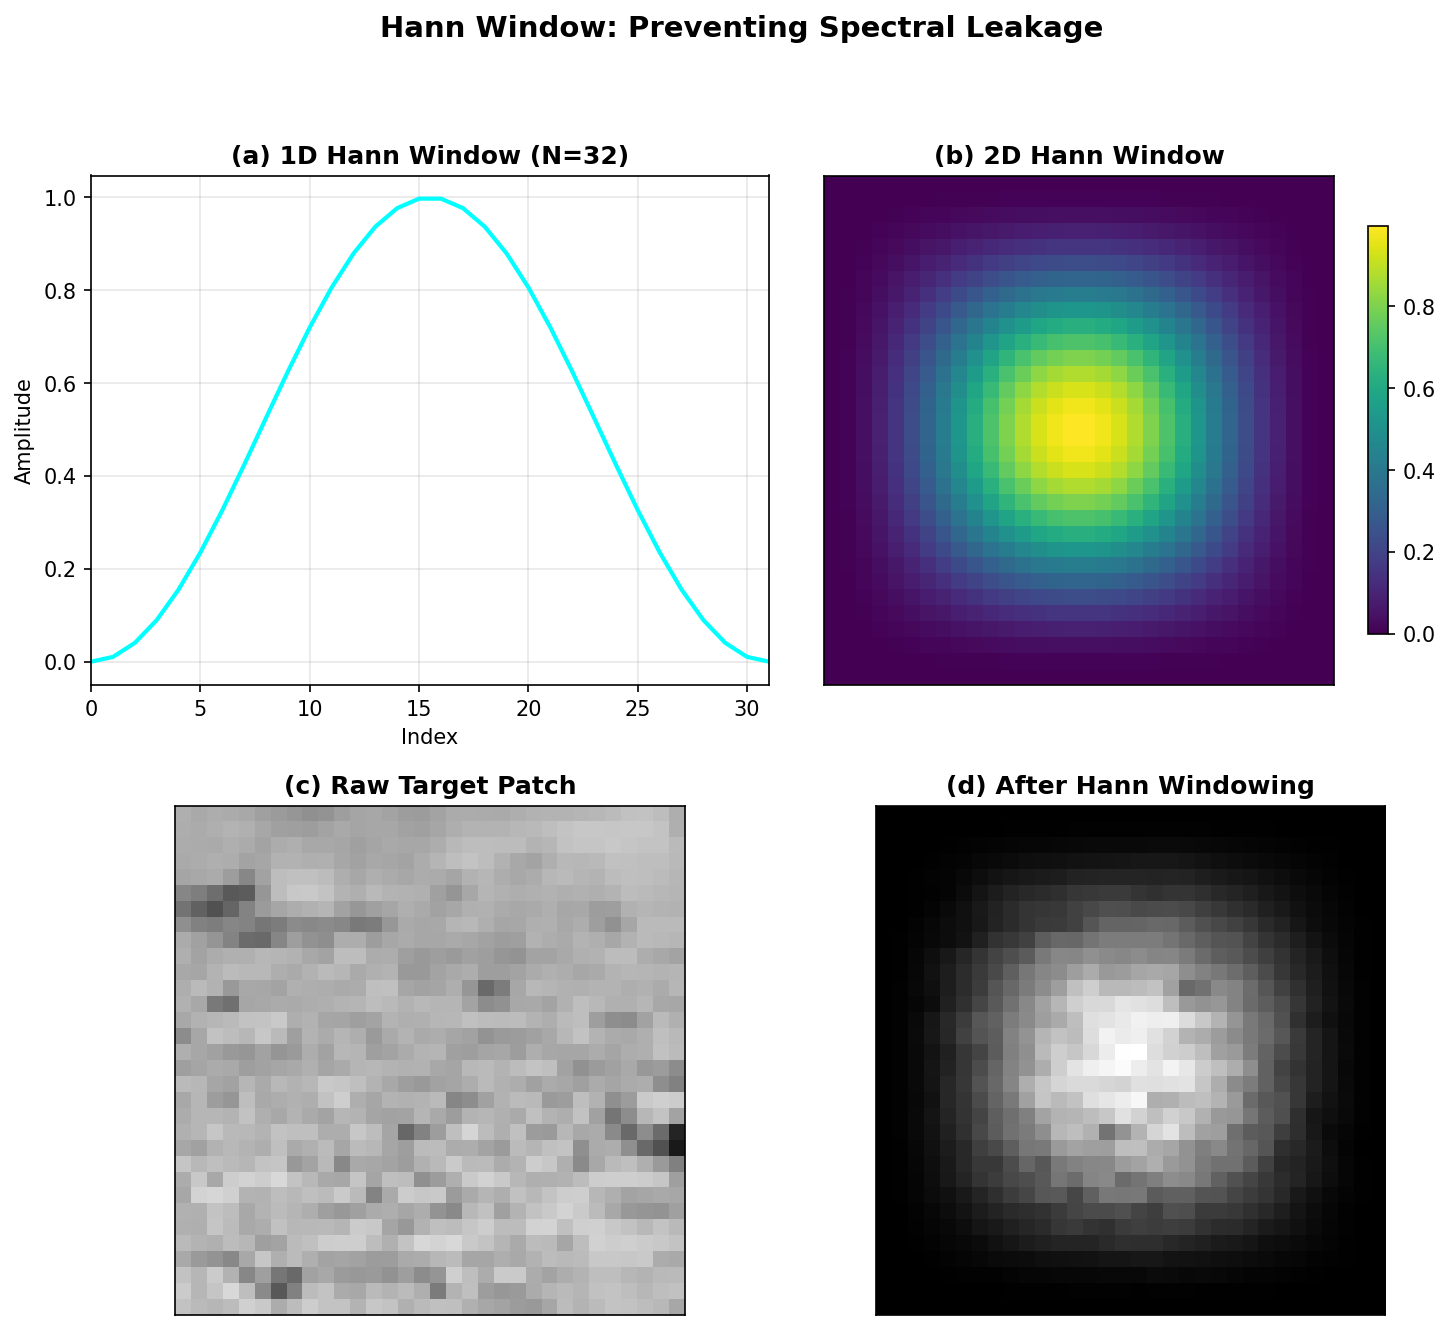
\includegraphics[width=\textwidth]{fig_pres_hann_effect.png}
    \caption{Hann window applied to a training patch. Spectral leakage is suppressed by tapering the patch edges to zero.}
    \label{fig:hann}
  \end{minipage}
  \hfill
  \begin{minipage}[b]{0.48\textwidth}
  \centering
    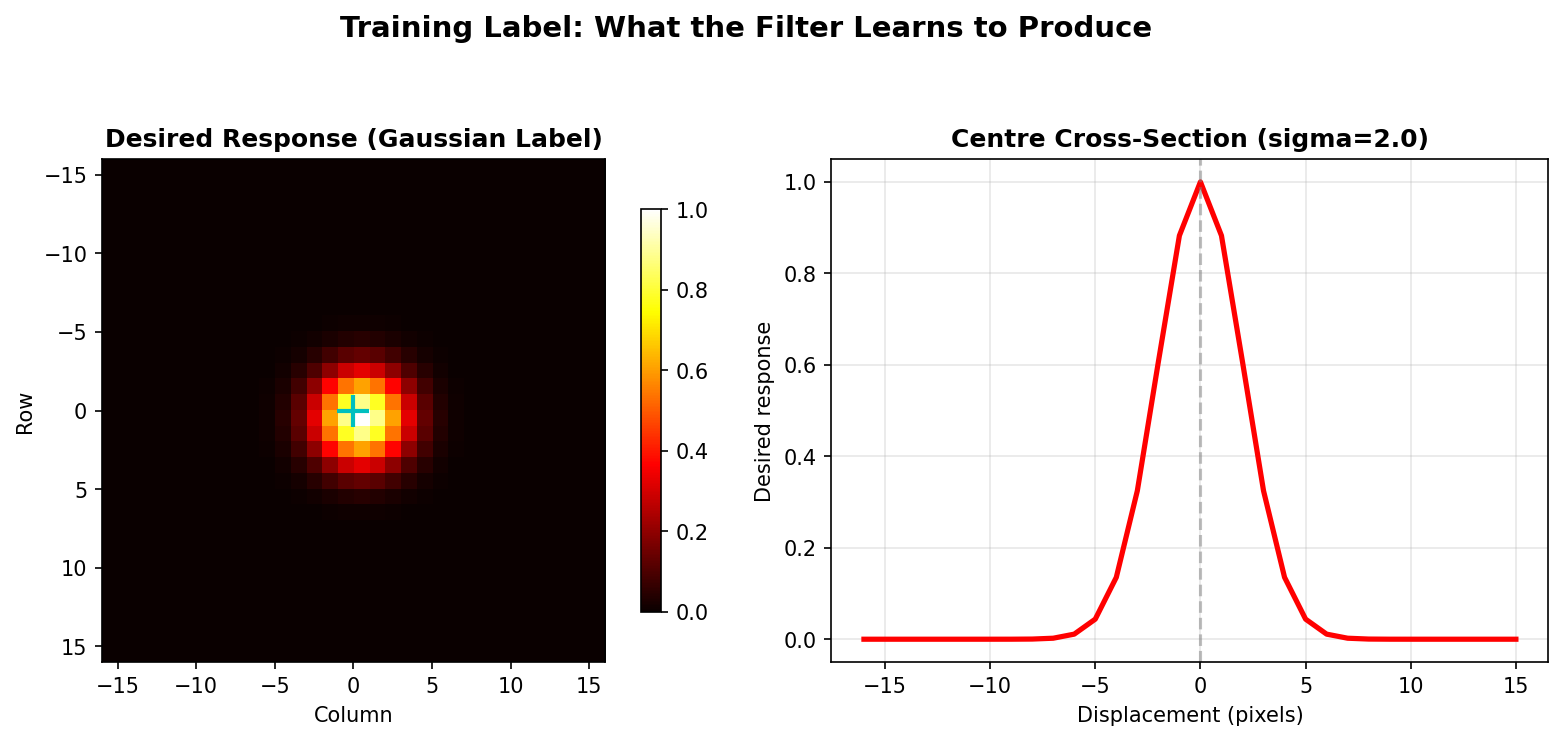
\includegraphics[width=\textwidth]{fig_pres_gaussian_label.png}
    \caption{2D Gaussian desired response ($\sigma{=}2.0$) used as the training label. The peak at centre encodes the target location.}
    \label{fig:gaussian}
  \end{minipage}
\end{figure}

\subsection{Detection Phase}

Given a new frame, a $32 \times 32$ search patch $z$ centred at the last known target location is extracted and processed:

\begin{enumerate}
    \item Apply the 2D Hann window: $z_w = z \odot (w \otimes w)$
    \item Compute $\hat{Z} = \mathcal{F}_\text{2D}(z_w)$
    \item Compute the response map in the frequency domain:
    \begin{equation}\label{eq:response}
    \hat{R}[k] = \overline{\hat{X}[k]} \cdot \hat{Z}[k] \cdot \hat{\alpha}[k]
    \end{equation}
    \item Compute the spatial response map: $R = \mathcal{F}^{-1}_\text{2D}(\hat{R})$
    \item Locate the peak of $R$ — its $(row, col)$ offset from the patch centre gives the target displacement.
\end{enumerate}

\section{NCC -- KCF Three-Frame Demo Pipeline}

A software demonstration pipeline was developed in \texttt{scripts/kcf\_demo\_visual.py} implementing the handoff from NCC-based acquisition to KCF-based tracking:

\begin{itemize}
    \item \textbf{Frame 1 (Training):} The user clicks to select the target centre in the reference image. A $32\times32$ patch is extracted, and KCF training is performed to compute $\hat{\alpha}$.
    \item \textbf{Frame 2 (NCC Acquisition):} NCC is computed between the template and a second real image. A valid-region mask ensures the search window stays within image boundaries. The peak of the normalised correlation map gives the initial target estimate in Frame~2.
    \item \textbf{Frame 3 (KCF Tracking):} A synthetic third frame is generated using \texttt{numpy\allowbreak.roll()} to introduce a controlled pixel-level shift. KCF detection (Equation~\ref{eq:response}) is run on the patch centred at the NCC result, and the response map peak provides the refined target position.
\end{itemize}

\par Figures~\ref{fig:frame1}--\ref{fig:frame3} illustrate the three-stage pipeline on a real image pair.

\begin{figure}[ht]
\centering
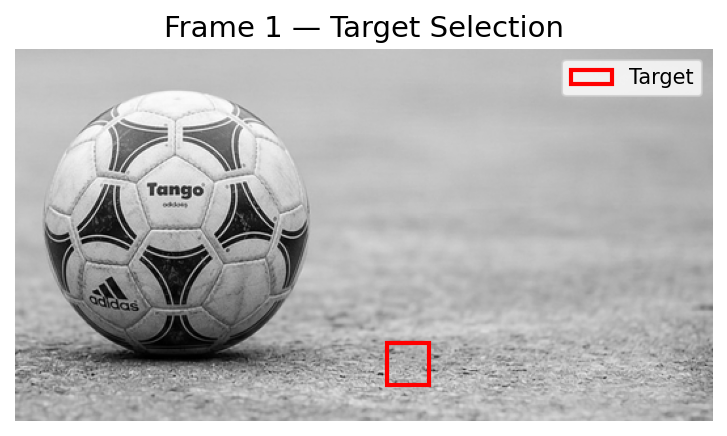
\includegraphics[width=0.7\textwidth]{fig_frame1_target.png}
\caption{Frame 1: User-selected target region (green bounding box). The $32\times32$ patch centred here is used for KCF training.}
\label{fig:frame1}
\end{figure}

\begin{figure}[ht]
  \centering
  \begin{minipage}[b]{0.48\textwidth}
  \centering
    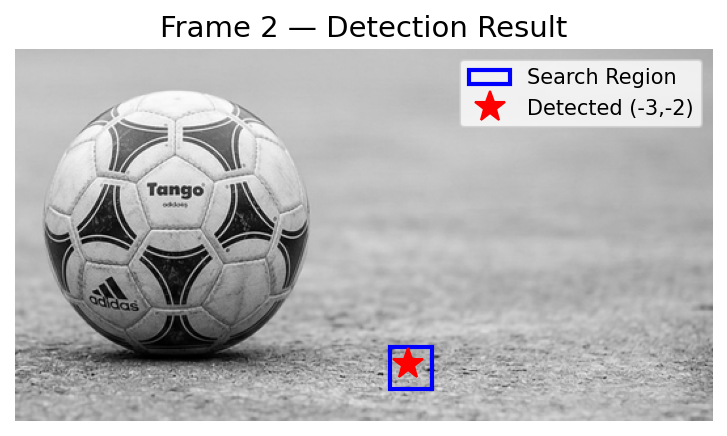
\includegraphics[width=\textwidth]{fig_frame2_search.png}
    \caption{Frame 2: NCC search result. The heatmap shows correlation scores across the search region.}
    \label{fig:frame2}
  \end{minipage}
  \hfill
  \begin{minipage}[b]{0.48\textwidth}
  \centering
    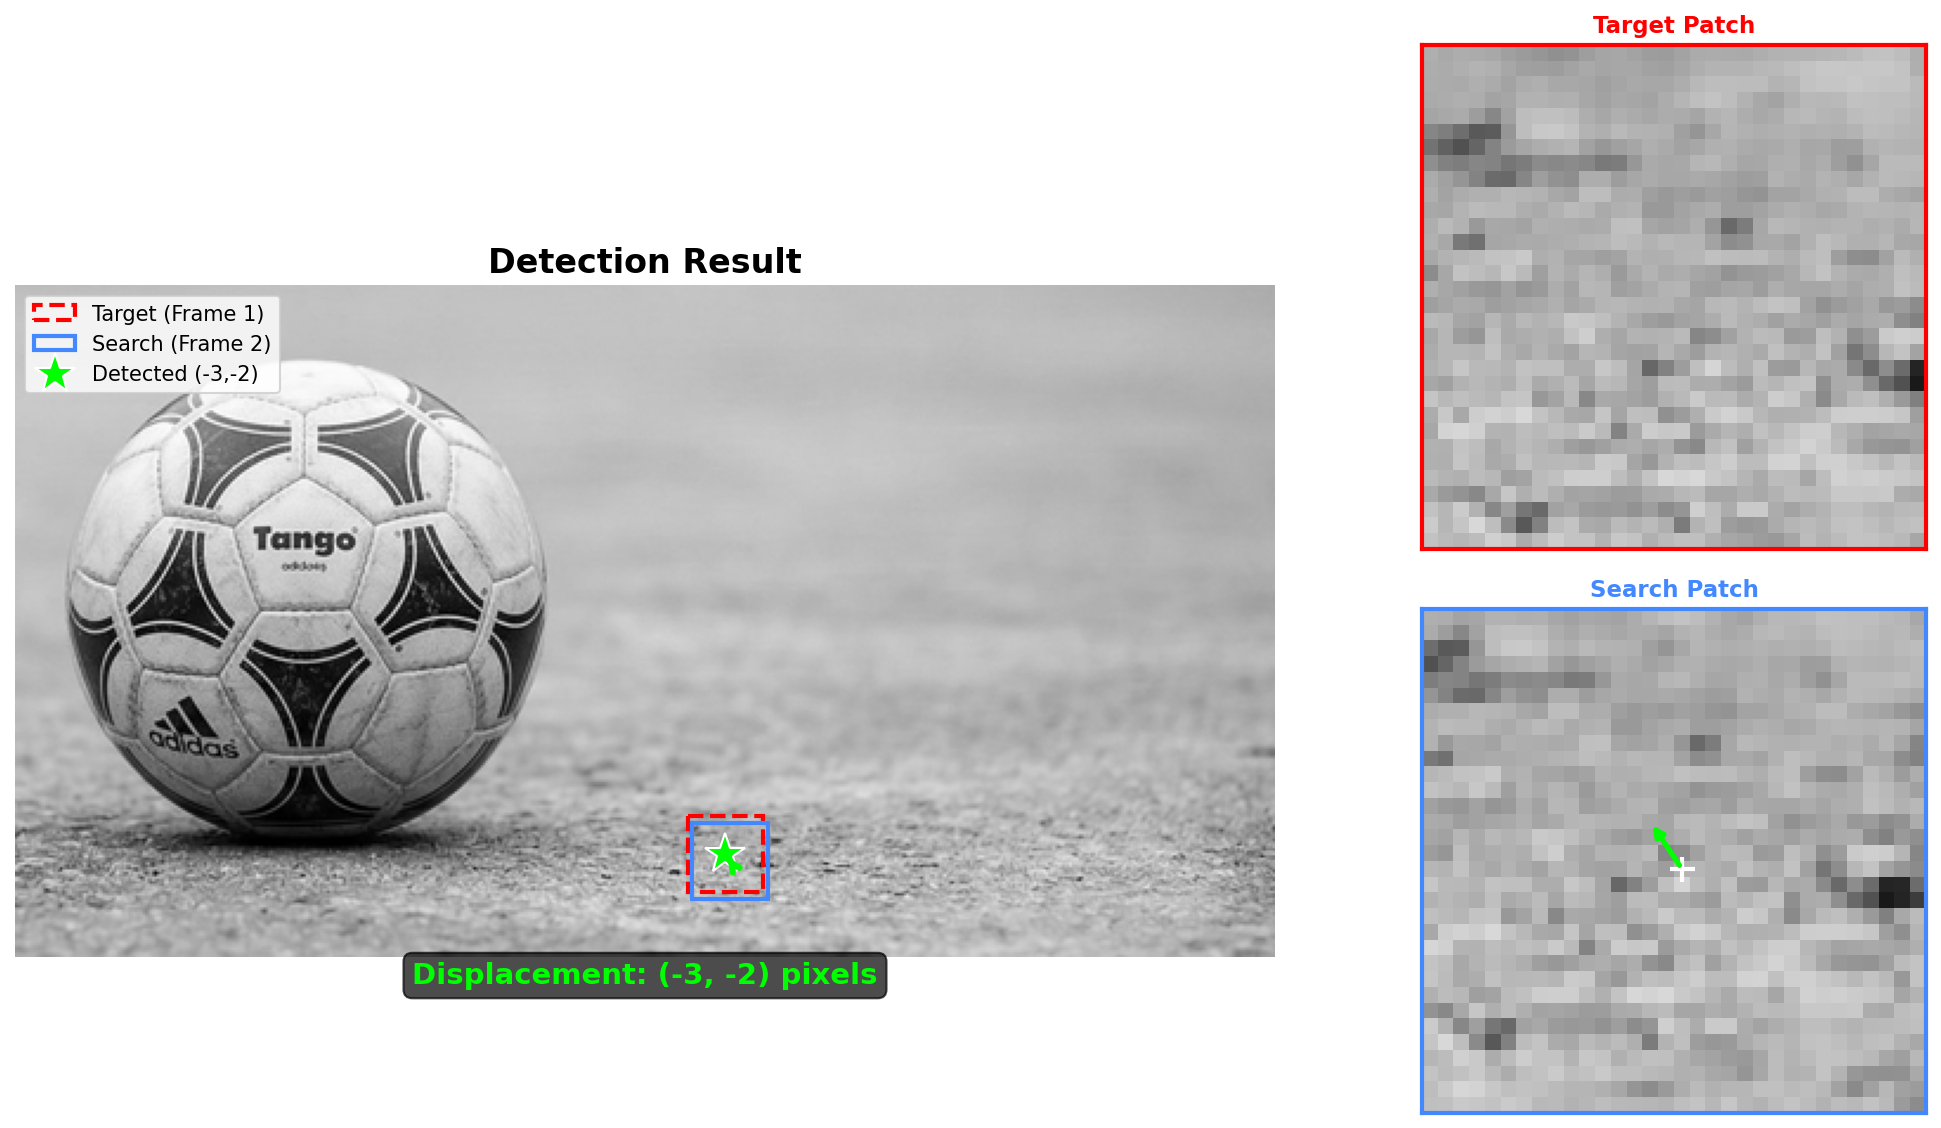
\includegraphics[width=\textwidth]{fig_pres_detection_result.png}
    \caption{Frame 3: KCF detection result on the NCC-initialised patch. The bounding box marks the refined target position.}
    \label{fig:frame3}
  \end{minipage}
\end{figure}

\section{RTL Hardware Architecture}

\subsection{Top-Level FSM: \texttt{kcf\_detect\_top.sv}}

The top-level RTL module \texttt{kcf\_detect\_top.sv} implements a 7-stage synchronous FSM that orchestrates the full KCF detection pipeline. Table~\ref{tab:fsm} lists each stage with its approximate cycle count.

\begin{table}[ht]
\centering
\caption{KCF Detection FSM Pipeline Stages}
\vspace{0.2cm}
\label{tab:fsm}
\begin{tabular}{|l|l|l|l|}
\hline
\textbf{Stage} & \textbf{State Name} & \textbf{Cycles (approx.)} & \textbf{Operation} \\ \hline
0 & \texttt{S\_IDLE} & --- & Wait for \texttt{start} pulse \\ \hline
1 & \texttt{S\_HANN\_WIN} & 1024 & Element-wise Hann multiply \\ \hline
2 & \texttt{S\_FFT\_LOAD} & 32 & Load rows into FFT engine \\ \hline
3 & \texttt{S\_FFT\_RUN} & $\approx$5600 & 2D-FFT (32 row + 32 col FFTs) \\ \hline
4 & \texttt{S\_ELEM\_MUL} & 1024 & $\overline{\hat{X}} \cdot \hat{Z} \cdot \hat{\alpha}$ element-wise \\ \hline
5 & \texttt{S\_IFFT\_LOAD} & 32 & Load into IFFT engine \\ \hline
6 & \texttt{S\_IFFT\_RUN} & $\approx$5600 & 2D-IFFT (conjugate trick) \\ \hline
7 & \texttt{S\_PEAK\_RUN} & 1024 & Scan for peak position \\ \hline
  & \texttt{S\_DONE} & 1 & Latch output, assert \texttt{done} \\ \hline
\multicolumn{2}{|l|}{\textbf{Total}} & $\approx$\textbf{19{,}300} & $\approx$ \textbf{193 $\mu$s @ 100 MHz} \\ \hline
\end{tabular}
\end{table}

\par The \texttt{done} signal is a single-cycle pulse asserted in \texttt{S\_DONE}. The outputs \texttt{peak\_row}, \texttt{peak\_col}, \texttt{peak\_val}, and \texttt{target\_found} are latched combinatorially and held valid until the next \texttt{start} pulse.

\subsection{Building Blocks}

The RTL design is composed of the following parameterised modules:

\begin{itemize}
    \item \textbf{\texttt{butterfly.sv}} --- Single butterfly unit computing $(a + W \cdot b,\ a - W \cdot b)$ using Q8.8 fixed-point complex multiplication.
    \item \textbf{\texttt{twiddle\_rom\_32.sv}} --- Precomputed ROM of $W_N^k = e^{-j2\pi k/N}$ twiddle factors for $N=32$.
    \item \textbf{\texttt{fft1d\_32.sv}} --- Iterative Radix-2 DIT FFT engine for 32-point 1D transforms. Processes one butterfly per cycle; completes in 80 cycles.
    \item \textbf{\texttt{fft2d\_32.sv}} --- Row-column 2D-FFT. Applies \texttt{fft1d\_32} to all 32 rows then all 32 columns.
    \item \textbf{\texttt{ifft2d\_32.sv}} --- 2D-IFFT implemented using the conjugate trick (Section~\ref{sec:ifft}).
    \item \textbf{\texttt{hann\_rom\_32.sv}} --- ROM containing the 32-point Hann window coefficients in Q8.8.
    \item \textbf{\texttt{cconj\_mul.sv}} --- Complex conjugate multiplier: computes $\overline{A} \cdot B \cdot C$ for three Q8.8 complex operands.
    \item \textbf{\texttt{peak\_finder.sv}} --- Scans the $32\times32$ real-valued response map in 1024 cycles and outputs the $(row, col)$ of the maximum value.
\end{itemize}

\subsection{2D-FFT Implementation}

The 2D-FFT is computed via the separable row-column decomposition. For an input array $X[r][c]$ of size $N \times N$:

\begin{equation}
\mathcal{F}_\text{2D}(X) = \mathcal{F}_\text{col}\!\left(\mathcal{F}_\text{row}(X)\right)
\end{equation}

\noindent The \texttt{fft2d\_32} module first applies \texttt{fft1d\_32} to each of the 32 rows (yielding a row-transformed buffer), then applies \texttt{fft1d\_32} to each of the 32 columns of the intermediate result. Total cycle count is $2 \times 32 \times 80 = 5120$ cycles for the transform passes plus overhead for memory reads/writes.

\subsection{IFFT via Conjugate Trick}\label{sec:ifft}

Rather than implementing a separate IFFT datapath, the IFFT is computed by reusing the forward FFT engine with the following identity:

\begin{equation}\label{eq:ifft_trick}
\mathcal{F}^{-1}(X) = \frac{\overline{\mathcal{F}(\bar{X})}}{N^2}
\end{equation}

\noindent The implementation steps are: (1) conjugate the input array element-wise, (2) apply the forward 2D-FFT, (3) conjugate the result, (4) divide by $N^2 = 1024$ (implemented as an arithmetic right shift). This avoids duplicating the FFT butterfly logic and reduces LUT consumption.

\section{Q8.8 Fixed-Point Arithmetic and Scaling}

\subsection{Fixed-Point Format}

All arithmetic in the RTL pipeline uses the Q8.8 signed fixed-point format: 16-bit two's complement values with 8 integer bits and 8 fractional bits. One unit in the least significant position (ULP) represents $2^{-8} \approx 0.004$. The representable range is $[-128,\ +127.996]$.

\par The choice of Q8.8 is driven by the need to represent both the pixel values (range $[0, 255]$ after normalisation to $[0, 1]$, fitting in 8 fractional bits) and the FFT twiddle factors (range $[-1, +1]$, which require fractional bits).

\subsection{Precision Problem with Naive Two-Pass Scaling}

A standard 2D-FFT implementation applies a $1/N$ normalisation factor after each pass (row and column), resulting in a total $1/N^2 = 1/1024$ attenuation of the signal. In Q8.8, dividing all values by 1024 causes the response map peaks to round to zero, completely destroying the tracking output.

\subsection{Scaling Solution: Asymmetric FFT and Adaptive Pre-scaling}

Two complementary techniques are employed to solve the precision problem:

\begin{enumerate}
    \item \textbf{Asymmetric FFT Scaling:} The $1/N$ normalisation is applied only in the row-pass of the FFT, not the column-pass. The column-pass is unscaled. This gives a total attenuation of $1/N$ instead of $1/N^2$, preserving 5 more bits of precision in the response map.
    \item \textbf{Adaptive Filter Pre-scaling (constant $K$):} Before loading $\hat{\alpha}$ into the ROM, the Python training script computes a scale factor $K$ such that $\max|\hat{\alpha}| \times K < 120$ (just below the Q8.8 saturation limit of 127). All $\hat{\alpha}$ values are multiplied by $K$ before serialisation. The hardware response map is correspondingly scaled up by $K$, but since we only care about the \emph{location} of the peak (not its absolute magnitude), this does not affect tracking accuracy.
\end{enumerate}

Table~\ref{tab:params} summarises all key algorithm parameters used in both the software reference model and the RTL implementation.

\begin{table}[ht]
\centering
\caption{KCF Algorithm and Hardware Parameters}
\vspace{0.2cm}
\label{tab:params}
\begin{tabular}{|l|l|l|}
\hline
\textbf{Parameter} & \textbf{Value} & \textbf{Description} \\ \hline
$N$ & 32 & Patch side length (pixels) \\ \hline
\texttt{DATA\_WIDTH} & 16 & Fixed-point word width (bits) \\ \hline
\texttt{FRAC} & 8 & Fractional bits (Q8.8) \\ \hline
$\lambda$ & 0.01 & Ridge regression regularisation constant \\ \hline
$\sigma$ & 2.0 & Gaussian label bandwidth (pixels) \\ \hline
\texttt{SCALE} & Adaptive $K$ & Filter pre-scale factor \\ \hline
\texttt{CONF\_THRESHOLD} & Configurable & Minimum peak value for \texttt{target\_found} \\ \hline
Clock frequency & 100 MHz & Target operating frequency \\ \hline
Total latency & $\approx$19{,}300 cycles & Per-patch detection time ($\approx$193~$\mu$s) \\ \hline
\end{tabular}
\end{table}

\section{AXI Interface Design}

\subsection{Overview}

To integrate the KCF IP core into a standard SoC environment, an AXI wrapper module \texttt{kcf\_axi\_wrapper.sv} is designed. It exposes two standard AMBA AXI interfaces:

\begin{itemize}
    \item \textbf{AXI4-Stream Slave} (prefix \texttt{s\_axis\_}): receives a 32$\times$32 patch as a stream of 1024 consecutive 16-bit pixels, with \texttt{TLAST} asserted on the final beat.
    \item \textbf{AXI4-Lite Slave} (prefix \texttt{s\_axil\_}): provides a memory-mapped register interface for control and result readout.
\end{itemize}

\subsection{AXI4-Lite Register Map}

Table~\ref{tab:regmap} describes the six 32-bit registers exposed over AXI4-Lite (base address + offset).

\begin{table}[ht]
\centering
\caption{AXI4-Lite Register Map}
\vspace{0.2cm}
\label{tab:regmap}
\begin{tabular}{|l|l|l|l|}
\hline
\textbf{Offset} & \textbf{Register} & \textbf{Access} & \textbf{Description} \\ \hline
\texttt{0x00} & \texttt{CTRL} & W & Bit 0: write 1 to trigger \texttt{start} pulse \\ \hline
\texttt{0x04} & \texttt{THRESHOLD} & R/W & Bits [15:0]: confidence threshold for \texttt{target\_found} \\ \hline
\texttt{0x08} & \texttt{PEAK\_ROW} & R & Bits [4:0]: row of response peak (0--31) \\ \hline
\texttt{0x0C} & \texttt{PEAK\_COL} & R & Bits [4:0]: column of response peak (0--31) \\ \hline
\texttt{0x10} & \texttt{PEAK\_VAL} & R & Bits [15:0]: signed peak value (Q8.8) \\ \hline
\texttt{0x14} & \texttt{TARGET\_FOUND} & R & Bit 0: 1 if peak\_val $>$ threshold \\ \hline
\end{tabular}
\end{table}

\subsection{SoC Integration Protocol}

The standard software protocol for operating the KCF IP from a host processor is:

\begin{enumerate}
    \item Write the confidence threshold to \texttt{THRESHOLD} register.
    \item Initiate an AXI4-Stream DMA transfer of 1024 $\times$ 16-bit pixels from the frame buffer to the \texttt{s\_axis} port. The IP's \texttt{tready} is asserted when the core is in the idle state.
    \item Write 0x1 to the \texttt{CTRL} register to assert the \texttt{start} pulse after the patch has been fully received.
    \item Poll or interrupt-wait on the \texttt{PEAK\_ROW} register — alternatively, connect the \texttt{done} wire to a GPIO interrupt line.
    \item Read \texttt{PEAK\_ROW}, \texttt{PEAK\_COL}, \texttt{PEAK\_VAL}, and \texttt{TARGET\_FOUND}.
    \item Compute target displacement: $\Delta r = \text{PEAK\_ROW} - 16$, $\Delta c = \text{PEAK\_COL} - 16$.
\end{enumerate}

\par This interface is compatible with any AXI4-capable processor including RISC-V (e.g., RV32I soft cores implemented on the same FPGA device) and ARM Cortex-M/A series processors connected via an AMBA AXI interconnect fabric.

\section{Software Toolchain}

The following Python scripts were developed as part of this project:

\begin{itemize}
    \item \textbf{kcf\_demo\_visual.py} --- Interactive three-frame demo (NCC acquisition to KCF detection) with annotated OpenCV visualisation, demonstrating the full pipeline on real image pairs.
    \item \textbf{gen\_data\_32.py} --- Generates \texttt{alpha\_hat.mem}, \texttt{test\_patch\_32.mem}, and \texttt{test2\allowbreak\_patch\_32.mem} in hexadecimal format for Vivado/Icarus simulation via \texttt{\$readmemh}.
\end{itemize}

\section{Verification and Results}

\subsection{RTL Simulation}

The RTL design was simulated using Icarus Verilog. The testbench loads pre-computed patches and the reference filter from the \texttt{data/} directory, drives the \texttt{start} signal, and monitors the \texttt{done} pulse and peak output registers.

\par Figure~\ref{fig:waveform} shows the Vivado simulation waveform, confirming that the \texttt{done} signal is asserted after approximately 19{,}300 cycles and the peak coordinates are correctly latched.

\begin{figure}[ht]
\centering
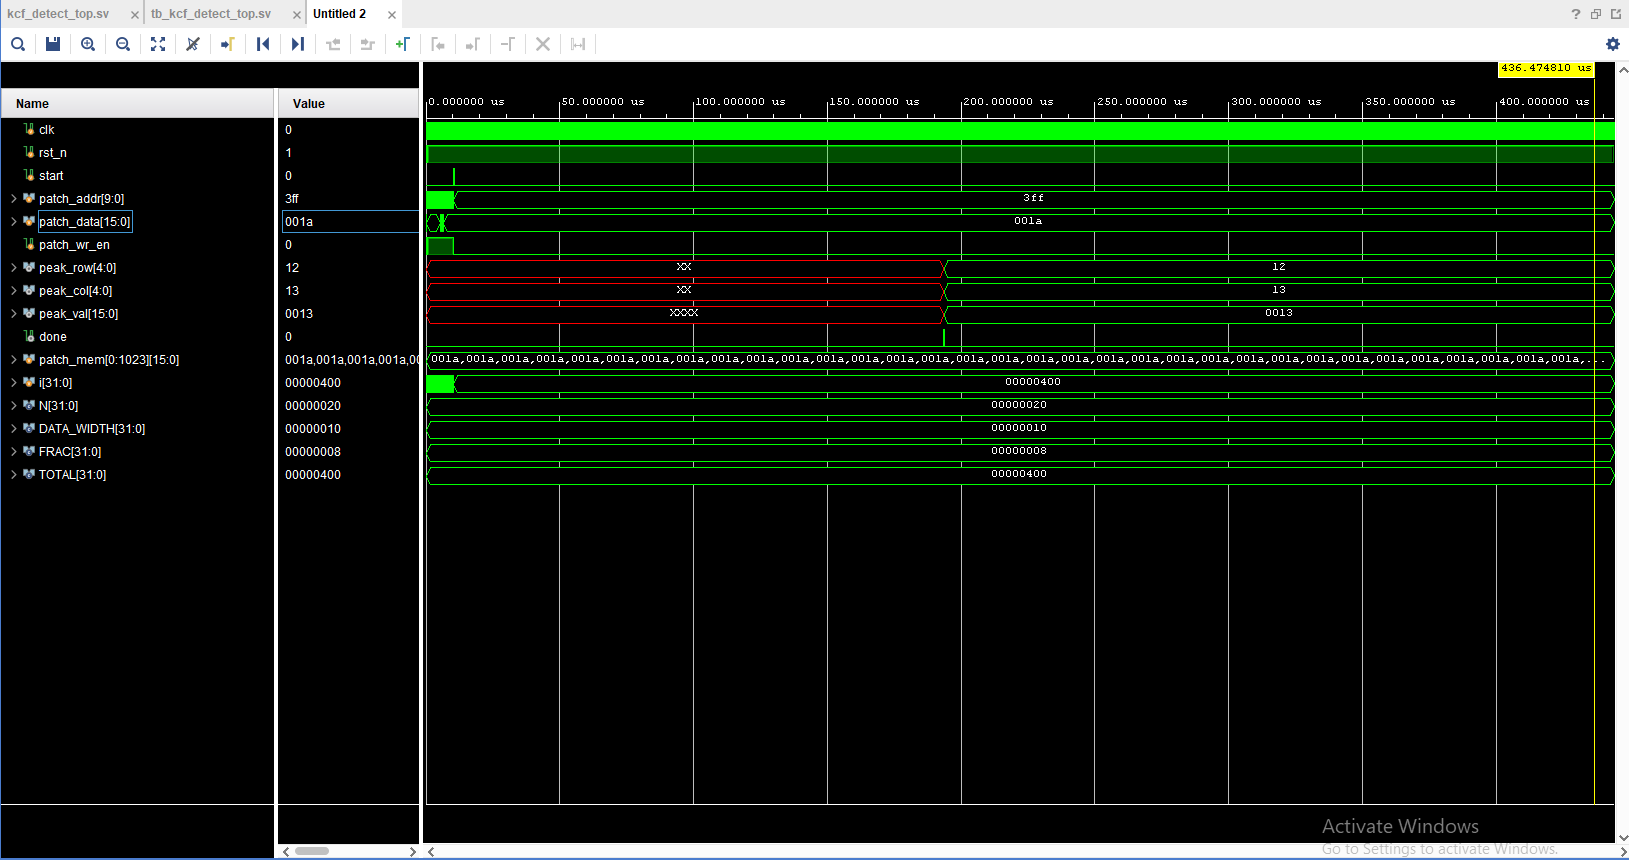
\includegraphics[width=\textwidth]{waveform.png}
\caption{Vivado simulation waveform showing the \texttt{done} pulse and output peak coordinates after the full KCF detection pipeline completes.}
\label{fig:waveform}
\end{figure}

\subsection{Hardware--Software Agreement}

The peak $(row, col)$ coordinates output by the RTL simulation were compared against the Python floating-point reference model for both test patches. Figure~\ref{fig:hwsw} shows the response maps from both implementations alongside the detected peak locations.

\begin{figure}[ht]
\centering
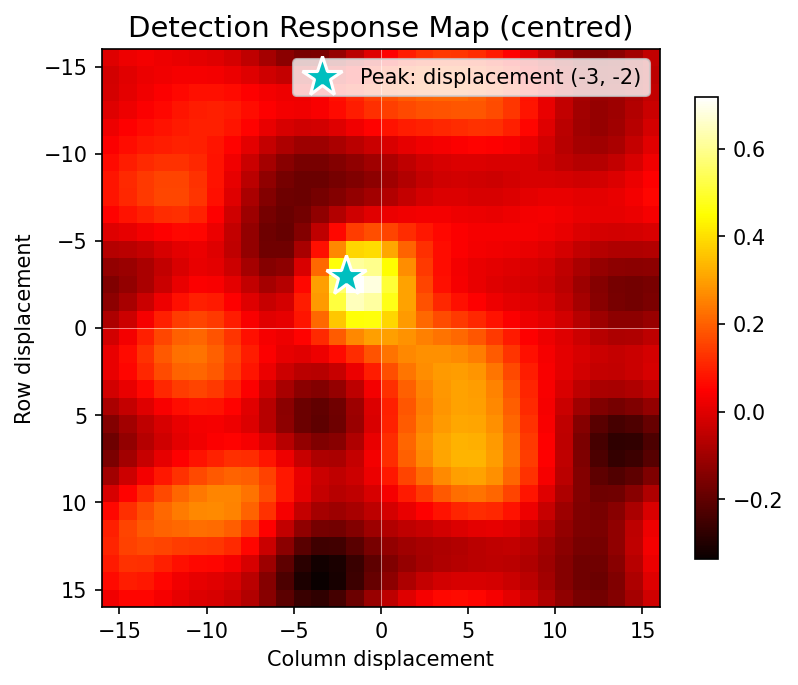
\includegraphics[width=0.8\textwidth]{fig_response_map.png}
\caption{KCF response map (2D heat-map) from the Python reference model. The peak at $(row{=}18, col{=}19)$ matches the RTL simulation output, confirming hardware--software agreement.}
\label{fig:hwsw}
\end{figure}

% ============================================================
%  CHAPTER 4: CONCLUSION
% ============================================================
\chapter{Conclusion}

This project presents a complete, synthesisable RTL implementation of the Kernelized Correlation Filter visual tracking algorithm in SystemVerilog. The design successfully demonstrates all core stages of the KCF detection pipeline:

\begin{itemize}
    \item A 7-stage FSM orchestrating Hann windowing, 2D-FFT, element-wise complex correlation, 2D-IFFT, and peak detection.
    \item A novel asymmetric FFT scaling scheme combined with adaptive filter pre-scaling that resolves the precision loss inherent to two-pass Q8.8 fixed-point FFT normalisation.
    \item The IFFT conjugate trick, which eliminates the need for a separate IFFT datapath by reusing the forward FFT hardware.
    \item An AXI4-Stream and AXI4-Lite wrapper providing a standard SoC-compatible interface.
    \item A Python software toolchain providing a floating-point reference model, test vector generation, and an interactive tracking demonstration.
\end{itemize}

\par Hardware--software agreement was verified between the Vivado RTL simulation and the Python reference model for both test patches. The full pipeline executes in approximately 19{,}300 clock cycles, corresponding to a detection latency of $\approx$193~$\mu$s at a 100~MHz clock, which is well within real-time video processing budgets for 30~fps ($\approx$33~ms per frame).

\par The design is validated at the register-transfer level and is ready for FPGA synthesis on the Xilinx Artix-7 (Nexys A7-100T) device using Vivado 2024.2. The AXI wrapper exposes the core as a plug-and-play IP block compatible with any AXI4-capable processor, positioning the design as a practical building block for embedded vision systems.

% ============================================================
%  CHAPTER 5: FUTURE PROSPECTS
% ============================================================
\chapter{Future Prospects}

Several extensions are planned or recommended to evolve this design toward a production-ready embedded tracking IP:

\begin{itemize}
    \item \textbf{FPGA Synthesis and Timing Closure:} Synthesise the current RTL on the Artix-7 XC7A100T device and report LUT, flip-flop, BRAM, and DSP48 utilisation. Close timing at 100~MHz and evaluate the maximum achievable frequency.
    \item \textbf{SoC Integration via AXI Interconnect:} Connect the KCF IP core to a RISC-V or ARM soft processor on the same FPGA device using the AXI4-Lite and AXI4-Stream interfaces designed in Chapter~3. This enables a complete embedded tracking system with host control.
    \item \textbf{Higher Resolution Support (64$\times$64):} Extend the FFT engine to support 64$\times$64 patches (6-stage Radix-2 DIT) to improve tracking accuracy on larger targets and enable operation at standard video resolutions.
    \item \textbf{Gaussian Kernel Support:} Implement the full Gaussian (RBF) kernel by adding a hardware exponential Look-Up Table (LUT) for $e^x$. This extends the feature space and improves robustness to appearance changes.
    \item \textbf{Online Model Update:} Add a hardware update path that combines the current filter with a new one via a learning rate $\eta$: $\hat{\alpha}_\text{new} = (1-\eta)\hat{\alpha}_\text{old} + \eta\hat{\alpha}_\text{frame}$. This allows the tracker to adapt to gradual appearance changes without host CPU intervention.
    \item \textbf{Camera / HDMI Input Pipeline:} Integrate a camera input module (MIPI CSI-2 or OV7670 parallel) and HDMI output module to create a fully self-contained real-time tracking demonstration system on the Nexys A7 board.
\end{itemize}

\pagebreak
\nocite{danelljan2014}
\addcontentsline{toc}{section}{References}
\bibliographystyle{IEEEtran}
\bibliography{reference_endterm}

\end{document}
